% !TEX encoding = UTF-8 Unicode
%!TEX root = main.tex
% !TEX spellcheck = en-US
%%=========================================


%%%%%%%%%%%%%%%%%%%%%%%%%%%%%%%%%%%%%%%%%%%%%%%%%%%%%%%%%%%%%%%%%%%%%%%%%%%%%%%%
\chapter{Implementation}
\label{ch:implementation}


The library is written in C++, with standard C++14 dialect. The reader is expected to have a fair understanding of C++, and being familiar with standard C++11 dialect or newer is recommended. Detailed explanations of the C++ programming language is not presented here. Refer to any C++ reference (e.g. \citet{stroustrup2013c++}) for more details.


%%%%%%%%%%%%%%%%%%%%%%%%%%%%%%%%%%%%%%%%%%%%%%%%%%%%%%%%%%%%%%%%%%%%%%%%%%%%%%%%
\section{Data Structures}
\label{sec:data_structures}


A set of data structures is commonly used by the runtime system. Apart from the C++ Standard Template Library (STL), the most notable data structures are \textit{intrusive containers}, \textit{concurrent queues}, and \textit{mutual exclusion locks}.


%%%%%%%%%%%%%%%%%%%%%%%%%%%%%%%%%%%%%%%%
\subsection{Intrusive Containers and Pointers}


Intrusive containers, just as any other containers, stores some kind of data in some sort of way. The difference is how the container stores the necessary data used to organize the data. A non\hyp{}intrusive container is responsible for storing the necessary data, while for an intrusive container the elements are responsible for storing the necessary data. In other words, the element becomes ``aware'' of being a part of the intrusive container. Usually, intrusive containers are implemented with the elements having \textit{hooks} as data members. These hooks contains all the necessary data used by the intrusive container to store the elements. 

An intrusive pointer is the intrusive equivalent of a smart pointer with shared ownership, releasing a dynamically allocated object when all owners have released the pointer. The owner counter is stored in the object rather in the pointer.

Intrusive containers and pointers offers better performance compared to non\hyp{}intrusive containers, as they minimize memory allocations and better memory locality. Intrusive containers and pointers are however much less maintainable, and are much harder to modularize.

Boost Intrusive containers and Boost Intrusive pointers are used as the implementation of intrusive containers and pointers.


%%%%%%%%%%%%%%%%%%%%%%%%%%%%%%%%%%%%%%%%
\subsection{Concurrent Queues}


Concurrent queues are queues which are safe to use concurrently, often denoted as \textit{thread safe}. The most common approach is taking a non\hyp{}thread safe queue and enforcing mutual exclusion around the critical regions. This approach however is not desirable, as it has very low throughput in multiprogrammed programs.

Concurrent queues often differentiate between single or multiple producers and consumers. Producers are processes which insert elements into the queue, and consumers are processes which remove elements from the queue. The runtime system uses the variants \textit{single\hyp{}producer\hyp{}multiple\hyp{}consumer} (SPMC) queues and \textit{multiple\hyp{}producer\hyp{}single\hyp{}consumer} (MPSC) queues.

A SPMC queue is used as a double\hyp{}ended queue for work\hyp{}stealing, implemented with the Chase\hyp{}Lev algorithm \citep{chase2005dynamic} combined with efficient work\hyp{}stealing for weak memory models \citep{le2013correct}.

A MPSC queue is used by schedulers to signal other schedulers a work process is to be rescheduled on the corresponding scheduler, implemented with the algorithm presented by \citet{vyukov2014intrusive}. 


%%%%%%%%%%%%%%%%%%%%%%%%%%%%%%%%%%%%%%%%
\subsection{Mutual Exclusion Locks}


Creating a complete non\hyp{}blocking system is most of the times impossible for a multiprogrammed programs. Sometimes resorting to mutual exclusion in critical regions is unavoidable. Different types of locks is suitable for different situations. Whether the lock is often contested, meaning multiple kernel\hyp{}threads are trying to acquire the lock simultaneously, and if the lock is held for a longer period of time or not, will affect the performance. 

\Citet[page 196--199]{brown2007c++csp2} performs a case study on different mutexes, describing various mutex algorithms and provides a benchmark and analysis of their performance. The conclusion from the case study is that for low contested, short\hyp{}term held mutexes, spinlocks yields best performance regarding low latency. 

For multiprocessor architectures, the \textit{test\hyp{}and\hyp{}test\hyp{}and\hyp{}set} (TTAS) spinlock is generally favorable as it causes less memory contention than the standard spinlock. Instead of constantly trying to test\hyp{}and\hyp{}set the lock, it waits until the lock appears free. Different variants of the TTAS spinlock includes constant/exponential backoff during contention and cache friendly atomic operations.

For most inter\hyp{}process runtime procedures, a TTAS spinlock with exponential backoff during contention is used. For idle schedulers waiting, the standard \lstinline[style={CustomC++}]|std::mutex| lock is used.


%%%%%%%%%%%%%%%%%%%%%%%%%%%%%%%%%%%%%%%%%%%%%%%%%%%%%%%%%%%%%%%%%%%%%%%%%%%%%%%%
\section{Runtime System Implementation}
\label{sec:runtime_system_implementation}


The runtime systems consists of two major implementation parts: implementation of lightweight processes, and implementation of a runtime scheduler.

Processes are implemented as user\hyp{}threads, and are called \textit{contexts} in the runtime. Processes uses contexts as its back end, meaning processes represent a meaningful part of computation while contexts represent the actual processor state of the computation. At runtime, the scheduler manipulates contexts when transferring control of execution between processes. 

The runtime differentiates between three types of contexts, and if a context is dynamic or static, i.e. a context can migrate between schedulers or not:

\begin{enumerate}[topsep=0em,itemsep=-1em,partopsep=0.5em,parsep=1em]
    \item \textbf{Main context} -- context of a kernel\hyp{}thread. When the main context returns, the corresponding kernel\hyp{}thread terminates. Main contexts are static; they cannot migrate between schedulers.
    \item \textbf{Scheduler context} -- context of the scheduler. The scheduler context only returns when the main program exits. Scheduler contexts are static; they cannot migrate between schedulers.
    \item \textbf{Work context} -- context of a work process. Work contexts are dynamic; they can migrate between schedulers.
\end{enumerate}

The initialization procedure of the runtime system is invoked with the first call to the scheduler. Given there are $N$ online logical processor cores, the procedure spawns $N-1$ additional kernel\hyp{}threads, as the initial main kernel\hyp{}thread is included. A scheduler is initialized for each kernel\hyp{}thread, representing the runtime environment for the corresponding thread. Schedulers are accessed via thread local static methods, which point to the scheduler object.

The initial main context, in other words context of the \texttt{main()} function, is special. It is the only context which represents some productive work of the running program, but cannot migrate between schedulers. All other main contexts (from the other spawned kernel\hyp{}threads) only joins the scheduler context, and operates invisible to the programmer. The initial main context cannot migrate because it is calling the runtime constructors. When the main context returns, the destructors are called for the corresponding runtime objects, such as the scheduler. If the initial main context where to migrate and return on an kernel\hyp{}thread other than its origin, the runtime cleanup would result in erroneous behaviour.

When the initial main context returns, the cleanup procedure of the runtime system is invoked if and only if the initialization procedure has been invoked previously.

Only the scheduler for which the initial main context resides on will begin as running. All other initialized schedulers will begin as idle.

\Cref{fig:runtime_overview} displays a rough outline of how the contexts, user\hyp{}threads and kernel\hyp{}threads are organized relative to each other. Note that the number of work contexts on each scheduler are zero\hyp{}or\hyp{}more, but the accumulative sum of all work contexts on all schedulers equals $M$.

\begin{figure}[h!]
    \centering
    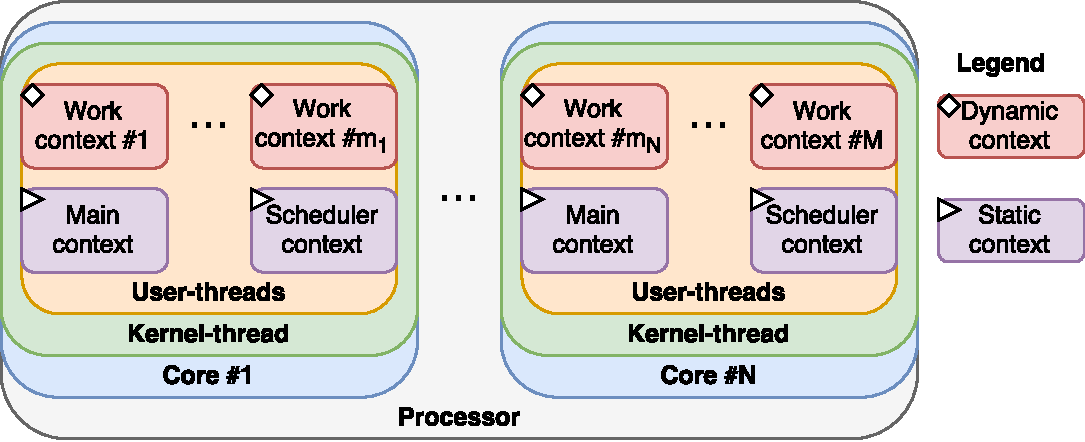
\includegraphics[width=0.9\linewidth]{fig/runtime_overview}
    \caption{Overview of the runtime system with $M$ work contexts, given $N$ online processor cores.}
    \label{fig:runtime_overview}
\end{figure}


%%%%%%%%%%%%%%%%%%%%%%%%%%%%%%%%%%%%%%%%
\subsection{Processes}
\label{subsec:process_implementation}


Processes are a vital part of ProXC++. As stated many times before, processes represents some kind of computation of the total program, which in code translates to running a function concurrently with the rest of the system. Constructing a process requires to supply a function pointer and its corresponding arguments. The process object constructs a context object out the function pointer and arguments, and stores an intrusive pointer to the context object as a data member. In other words, the process is no more than an opaque type to a context object. The programmer implicitly creates new contexts through processes, while the scheduler under the hood operates on the contexts. See \cref{lst:process_type} for reference.

\begin{lstfloat}
\begin{lstlisting}[caption={Minimal process type.}, label={lst:process_type}, style={CustomC++}, xleftmargin={2em}]
class Process {
private:
    using CtxPtr = boost::intrusive_ptr<proxc::Context>;
    CtxPtr ctx_ptr_{ nullptr };
public:
    template<typename Fn, typename... Args>
    Process(Fn && fn, Args &&... args);
};
\end{lstlisting}
\end{lstfloat}

The context objects represent the execution state of the computation. Each context object contains an execution context, which is the actual execution state of the computation. The execution context is implemented by the Boost Context library, which encapsulates context switching and manages the associated contexts stack. Note that a context object refers to the context type defined by the runtime system, and execution context refers to the Boost Context object which defines the actual processor state.

The context object does not implement much functionality, other than wrapping the execution context state with additional control structure data and intrusive data members. The functionality is implemented in the scheduler, which is explained in further detail in \cref{subsec:scheduler_implementation}.

Execution contexts can either create a context of the current running execution context, or takes a function pointer of the type \lstinline[style={CustomC++}]|void(void*)|. Transfer of control flow between execution contexts is done by calling another execution context with the overloaded \lstinline[style={CustomC++}]|void* operator()(void*)| method. Parameter passing is possible through void pointer casting. When transferring control to another execution context, an optional pointer can be passed. If this is the first transfer of control to the execution context, the parameter will be passed as the void pointer argument for the function. Else, the void pointer will be passed as the return value of the transfer of control operator.

\Cref{lst:transfer_control_execution_contexts} gives an example of how execution contexts work. An execution context of the current running context is made, as well as an execution context of a lambda function. The output of the code snippet will print \texttt{main} and \texttt{work} in that order. Refer to the Boost Context documentation for more thorough explanation of the execution context implementation \citep{kowalke2017boost}.

\begin{lstfloat}
\begin{lstlisting}[caption={Transfer of control between execution contexts.}, label={lst:transfer_control_execution_contexts}, style={CustomC++}, xleftmargin={2em}]
using ex_ctx = boost::context::execution_context;
ex_ctx main_ctx{ex_ctx::current()};
ex_ctx work_ctx{[&main_ctx](void* vp){
    std::string* msg = static_cast<std::string*>(vp);
    std::cout << *msg << std::endl;
    // prints `main`
    std::string work_msg{"work"};
    // transfer of control to main_ctx
    main_ctx(static_cast<void*>(&work_msg));
    // never returns
}};
std::string main_msg{"main"};
// transfer of control to work_ctx
void* vp = work_ctx(static_cast<void*>(&main_msg));
std::string* msg = static_cast<std::string*>(vp);
std::cout << *msg << std::endl;
// prints `work`
\end{lstlisting}
\end{lstfloat}

When creating a context object, an enclosing entry function of the type \lstinline[style={CustomC++}]|void(void*)| is created, which calls the received function with its arguments. This entry function, called trampoline, handles the void pointer argument from the execution context, calls the process function, and calls the terminate procedure when the process function returns. This way, all terminating processes can be gracefully resolved by the trampoline invisible to the programmer. Entry functions are created with generic lambdas, allowing to create generic entry function calling over any type of function pointer and arguments. This is explained in further detail in \cref{subsec:scheduler_implementation}.

The context object contains the type of the context, the execution context, the entry function for the particular process, and a pointer to the parent scheduler. Each process also has its own spinlock, used when synchronizing on certain inter\hyp{}process synchronization. Additionally, control data used by the scheduler is stored in the context object, such as intrusive hooks and time points for timed suspension. See \cref{lst:context_type} for a stripped down version of the context class definition.

\begin{lstfloat}
\begin{lstlisting}[caption={Minimal context type.}, label={lst:context_type}, style={CustomC++}, xleftmargin={2em}]
class Context {
private:
    using ExCtxT = boost::context::execution_context;
    using EntryFn = delegate<void(void*)>;
    using TimePointT = std::chrono::steady_clock::time_point;
    ExCtxT ex_ctx_;
    EntryFn entry_fn_{ nullptr };
    proxc::Scheduler * scheduler_ptr_{ nullptr };
public:
    TimePointT time_point_{ TimePointT::max() };
    proxc::Alt * alt_{ nullptr };
    proxc::Spinlock splk_;
    /* impl defined */ wait_queue_{};
    /* intrusive data members */
};
\end{lstlisting}
\end{lstfloat}

FIXME wait queue.


%%%%%%%%%%%%%%%%%%%%%%%%%%%%%%%%%%%%%%%%
\subsection{Scheduler}
\label{subsec:scheduler_implementation}


The scheduler is the corner piece of runtime system. It has the sole responsibility of managing the different processes, including creating, scheduling, and synchronizing processes. The scheduler runs as its own context, invisible to the programmer.

When the scheduler is initialized by the runtime initialization procedure, the scheduler context enters the scheduler event loop. The scheduler event loop is where the scheduler context resides during the lifetime of the entire program.

A scheduler is implemented as a class object, consisting of context queues and process management logic. See \cref{lst:scheduler_type} for reference.

\begin{lstfloat}
\begin{lstlisting}[caption={Minimal scheduler type.}, label={lst:scheduler_type}, style={CustomC++}, xleftmargin={2em}]
class Scheduler {
private:
    struct Initializer;
    bool exit_{ false };
    proxc::Context* running_ptr_{ nullptr };
    proxc::Spinlock splk_;
    /* impl defined */ policy_;
    /* impl defined */ work_queue_{};
    /* impl defined */ sleep_queue_{};
    /* impl defined */ terminated_queue_{};
    /* impl defined */ remote_queue_{};
public:
    static proxc::Scheduler* self();
    static proxc::Context* running();
};
\end{lstlisting}
\end{lstfloat}


%%%%%%%%%%%%%%%%%%%%%%%%%%%%%%%%%%%%%%%%
\subsubsection{Scheduler Initialization}


The scheduler has two static methods: \lstinline[style={CustomC++}]|self()| and \lstinline[style={CustomC++}]|running()|. The \lstinline[style={CustomC++}]|self()| method returns a pointer to the scheduler object which is the parent scheduler for the current running kernel\hyp{}thread, and can be called from any context. The \lstinline[style={CustomC++}]|running()| method returns a pointer to the context object currently running on the kernel\hyp{}thread, and can be called from any context.

The \lstinline[style={CustomC++}]|self()| method is the starting point of the runtime system, for which the first call to will trigger the initialization procedure. The method contains a static thread local variable of the scheduler initializer object, which is a Schwarz counter. A Schwarz counter, also known as a nifty counter, is a C++ idiom for ensuring a non\hyp{}local static object is initialized before its first use and destroyed only after last use of the object, where the non\hyp{}local static object in this case is the scheduler object. 

The first call to the scheduler initializer constructor on each kernel\hyp{}thread will initialize the scheduler object for the corresponding kernel\hyp{}thread, and simultaneously set its static thread local pointer member to the scheduler object. This static thread local pointer is the pointer which is returned by \lstinline[style={CustomC++}]|self()| method. Additionally, the \lstinline[style={CustomC++}]|running()| method returns the \lstinline[style={CustomC++}]|running_ptr_| member from the returned scheduler object, which is retrieved by the \lstinline[style={CustomC++}]|self()| method.

\begin{lstfloat}
\begin{lstlisting}[caption={Static scheduler methods.}, label={lst:static_scheduler_methods}, style={CustomC++}, xleftmargin={2em}]
// Schwarz counter
struct Scheduler::Initializer {
    thread_local static Scheduler* self_{ nullptr };
    thread_local static std::size_t counter_{ 0 };
    Initializer() {
        if (counter_++ == 0) { 
            /* initialize scheduler */ 
            /* member self_ is set */
        }
    }
    ~Initializer() {
        if (--counter_ == 0) { /* destroy scheduler */ }
    }
};
Scheduler* Scheduler::self() {
    thread_local static Initializer init;
    return Initializer::self_;
}
Context* Scheduler::running() {
    return Scheduler::self()->running_;
}
\end{lstlisting}
\end{lstfloat}


%%%%%%%%%%%%%%%%%%%%%%%%%%%%%%%%%%%%%%%%
\subsubsection{Process Queues}


From \cref{lst:scheduler_type} a total of five queues are used by the scheduler for process management: \textit{ready}, \textit{work}, \textit{sleep}, \textit{terminated} and \textit{remote} queue. 

The ready queue is called a scheduling policy, or just policy for short. The scheduling policy is an abstraction for the scheduler, for which ready processes are enqueued to and ready processes to resume are dequeued from. The scheduling policy is responsible to store the ready processes, and how and in which order the processes are enqueued and dequeued is up to the implementation of the scheduling policy. The default policy, which is hard coded as of now, is the work stealing policy. However, any type of scheduling policy could be implemented, such as round robin. Following the algorithm described in \cref{subsec:work_stealing_algorithm}, the queue is implemented as a combination of a double\hyp{}ended queue, deque for short, and a doubly linked list. The deque is used for dynamic processes and the doubly linked list is used for static processes. This is to avoid static processes from being stolen by other schedulers. The deque has two distinct ends called \textit{top} and \textit{bottom}. Enqueueing and dequeueing a dynamic process to the dequeue pushes and pops the process from the bottom end, respectively. The doubly linked list acts as a FIFO queue. The work stealing commences when both the deque and the doubly linked list are empty. A deque from another scheduler is chosen at random, and a process is tried to be stolen from the top end. Pointers to all deques from all schedulers are stored in a static list. Note that work stealing is happening unbeknownst to the scheduler, as the scheduler only enqueues and dequeues processes to the scheduler policy. 

The work queue, which holds all processes the scheduler is the parent of, is implemented as an intrusive doubly linked list. The sleep queue, which holds all processes suspended until a time point, is implemented as an intrusive multiset\footnote{A multiset is an associative container that contains a set of objects, which allows multiple keys with the same values.}. The terminated queue, which holds all process which has terminated and can be destroyed, is implemented as an intrusive doubly linked list. Both work, sleep and terminated queues are only manipulated by a single scheduler and are therefore not thread\hyp{}safe, i.e. no other schedulers can access these queues safely.

The remote queue is a concurrent MPSC queue, where the managing scheduler is the consumer while any other schedulers are the producers. Whenever a scheduler reschedules a process and it is now the parent scheduler, the context is placed in the remote queue to the parent scheduler. The parent scheduler transitions proecsses in the remote queue and enqueues them in the scheduling polict. In essence, the remote queue is used to signal schedulers when their processes are to be rescheduled, since remote schedulers cannot safely access the scheduling policy.


%%%%%%%%%%%%%%%%%%%%%%%%%%%%%%%%%%%%%%%%
\subsubsection{Process States and Transitions}


The scheduler imposes a set of states for a process and how a process transitions between these states. An overview of the finite state machine of the states and transitions are shown in \cref{fig:context_states}. The different different process states implies the following:

\begin{itemize}[topsep=0em,itemsep=-1em,partopsep=0.5em,parsep=1em]
    \item \textbf{Ready} -- a newly created process always starts in the ready state. A ready process is enqueued to a ready queue and is ready to be resumed by the parent scheduler.
    \item \textbf{Running} -- a process is currently executing on a kernel\hyp{}thread.
    \item \textbf{Ended} -- a process has terminated and is enlisted in the terminated queue. An ended process is can be destroyed by the parent scheduler.
    \item \textbf{Suspend} -- a process is waiting indefinitely. An another process might reschedule the suspended process.
    \item \textbf{Sleep} -- a process is waiting until a given time point. A sleeping process is enlisted in the sleep queue and is rescheduled by the parent scheduler when the time point has expired or is rescheduled by an another process.
    \item \textbf{Join} -- a process is waiting for an another process to terminate. The joining process is enlisted in the wait queue of the process to terminate, and will be rescheduled when the process terminates.
    \item \textbf{Remote} -- a process is rescheduled by an another process which does not have the same parent scheduler. A remote ready process is enlisted in the remote queue.
\end{itemize}

Some observations can be made by the transition diagram in \cref{fig:context_states}. A ready process can only transition to running. Only a running process can terminate. A transition to and from running is the same as a context switch between two processes. Remote state can be seen as an intermediate ready state. When a running process transitions from running to one of the states suspend, sleep or join, the next transition must be ready state. A transition between the three states suspend, sleep or join cannot occur.

\begin{figure}[h!]
    \centering
    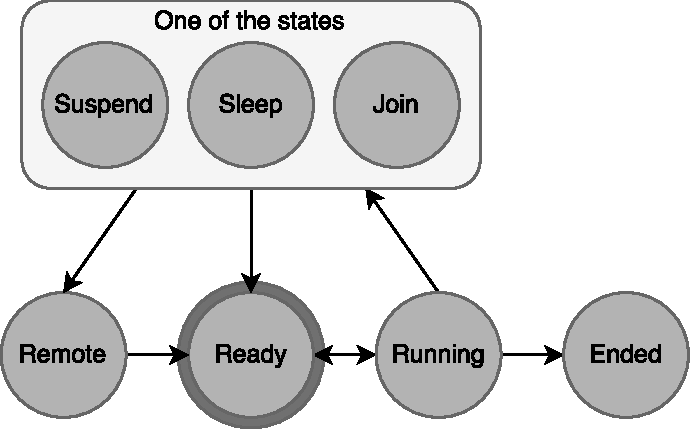
\includegraphics[width=0.7\linewidth]{fig/context_states}
    \caption{Finite state machine of states and transitions for a process.}
    \label{fig:context_states}
\end{figure}


%%%%%%%%%%%%%%%%%%%%%%%%%%%%%%%%%%%%%%%%
\subsubsection{Scheduler Functionality}


The scheduler implements a set of methods for manipulating processes, such as process management and inter\hyp{}process synchronization. It is important the scheduler implements the necessary functionality, as this forms the basis of what library features can be implemented. The follow functionality is available for a process:

\begin{itemize}[topsep=0em,itemsep=-1em,partopsep=0.5em,parsep=1em]
    \item \textbf{Process attaching and detaching} -- allows a process to be attached and detached to a scheduler, i.e. setting and removing a parent scheduler to a process.
    \item \textbf{Process rescheduling} -- allows a process to reschedule other processes.
    \item \textbf{Process suspension} -- allows a process to suspend execution, either indefinitely, for an another process, or until a given time point. 
    \item \textbf{Inter\hyp{}process synchronization} -- allows a process to synchronize on other processes, meaning the process waits for the other process to terminate.
    \item \textbf{Context switch operations} -- allows a process to perform certain operations immediately after context switch.
\end{itemize}

To further elaborate on the points above, attaching and detaching a process is necessary when work stealing. As all schedulers has a set of process of which it is responsible for, attaching a process is to register this responsibility. Detaching would unregister this responsibility. When a process migrates between two schedulers, the process must detach of its previous parent scheduler and attach to its new parent scheduler. 

a process rescheduling an another process requires checking whether they have the same parent scheduler or not. With the same parent scheduler, the process is enlisted directly to the ready queue. If different parent schedulers, the process is first enlisted to the remote queue, then enlisted to the ready queue when the parent schedulers transitions the process. If a rescheduled process was currently suspended with a timeout, the process is also removed from the sleep queue when enlisted to the ready queue.

Process suspension falls into two categories: waiting until some time point, or wait indefinitely. A process waiting until some time point enlists the process to the sleep queue. However, it is possible for other processes to reschedule the waiting process before the timeout occurs. A process waiting indefinitely may only be rescheduled by other processes.

Inter\hyp{}process synchronization, also called joining, allows for processes to wait for other processes to terminate. Each process has its corresponding spinlock, which is used to give mutual exclusion to the process termination flag. When a process terminates, the lock is acquired and the wait queue is checked. All processes enlisted to the wait queue is rescheduled and lastly the lock is released. On the other side when a process joining on an another process, the lock is first acquired and the termination flag is checked. If the termination flag is not set, the process enlists itself on the wait queue of the joining process, and the process suspends itself with releasing the lock. If the termination flag is set, the operation returns immediately. Note that it is safe for processes to access the wait queue as its guarded with mutual exclusion.

Context switch operations allows for processes to perform an action after the context switch has occurred. This is necessary when a process can only perform said action after itself has yielded execution. Currently, two operations requires a context switch operation: releasing a lock and rescheduling a process. Releasing a lock after a context switch is necessary when a process releasing a lock could result in the given process being rescheduled by an another process. An example of this is inter\hyp{}process synchronization. Rescheduling a process after a context switch is necessary when a process want to reschedule itself, such as processor yielding.


\FloatBarrier
%%%%%%%%%%%%%%%%%%%%%%%%%%%%%%%%%%%%%%%%
\subsubsection{Scheduler Event Loop}


The scheduler event loop is the where the entirety of the scheduler process is executing. The event loop consists of the following: check exit condition, process cleanup, process transitions, and process scheduling. See \cref{lst:scheduler_event_loop} for pseudo code reference.

What is important to note is that whenever the scheduler context switches to an another process, the scheduler process is enqueued to the ready queue before context switching. This ensures the scheduler is always available to context switch back to when running as a process. 

\begin{lstfloat}
\begin{lstlisting}[caption={Scheduler event loop pseudo code.}, label={lst:scheduler_event_loop}, style={CustomC}, xleftmargin={2em}]
while ( true ) {
    if (exit_condition()) {
        break;
    }
    // cleanup terminated contexts
    cleanup_terminated();
    // transition contexts to ready
    transition_remote(); // remote -> ready
    wakeup_sleep();      // sleep  -> ready
    // schedule ready context if any. Else, wait
    context = scheduling_policy.dequeue();
    if (context != nullptr) {
        // scheduler must always be available
        scheduling_policy.enqueue( scheduler_context );
        // context switch to ready process
        context.resume();
        // scheduler is now running
    } else {
        // sleep until first timeout or idle wakeup
        scheduling_policy.suspend_until( next_wakeup() );
    }
}
// scheduler is exiting, cleanup scheduler
scheduler_cleanup();
// lastly, context switch to main
main_context.resume();
// never returns
\end{lstlisting}
\end{lstfloat}

\FloatBarrier
%%%%%%%%%%%%%%%%%%%%%%%%%%%%%%%%%%%%%%%%%%%%%%%%%%%%%%%%%%%%%%%%%%%%%%%%%%%%%%%%
\section{Library Feature Implementations}

Library features provides the framework for the library for which are visible for the programmer. All features use the runtime system to implement its functionality, and this section explains this in further detail.


%%%%%%%%%%%%%%%%%%%%%%%%%%%%%%%%%%%%%%%%
\subsection{Timers}


The three types of timers described in \cref{subsec:timers_desgin} are represented through a common abstract class interface, shown in \cref{lst:timer_class_interface}. Instances of an egg or repeat timer converts the specified time duration to a time point, while the date timer already specifies a time point. This time point is stored in the base interface class. All timers support duration and time points from the standard library \lstinline[style={CustomC++}]|std::chrono|.

\begin{lstfloat}
\begin{lstlisting}[caption={Timer class interface.}, label={lst:timer_class_interface}, style={CustomC++}, xleftmargin={2em}]
class timer::Interface {
protected:
    using TimePointT = /* implementation defined */;
    TimePointT time_point_;
public:
    virtual void reset() = 0;
    virtual bool expired() = 0;
    bool operator<( Interface const & other ) const 
    { return time_point_ < other.time_point_; }
    TimePointT const & get() const { return time_point_; }
};
\end{lstlisting}
\end{lstfloat}

When a timer is supplied for a timed operation, the reset method is called. For the egg timer, a reset results in calculating new time point. For the repeat timer, the next periodic time point is calculated if expired, else the time point remains the same.

Multiple timers can be supplied for some operations, such as alting. Since timers have a static time point after a reset, the closest time point is chosen for timeout when there are multiple timers.

An explicit process suspension with a given timer is simply enlisting the process to the scheduler sleep queue with the corresponding time point. When the time point is reached, the scheduler will transition the process from the sleep queue to the ready queue. The time points are checked by the scheduler process in the scheduler event loop with the \texttt{Scheduler::wakeup\_sleep()} method. Suspending a process with a timer will immediately return if the time point is already reached.

A timed operation differs slightly from a timed suspension. Whenever the process waits for some event during the operation, the process is enlisted in the sleep queue. Now, one of two things may happen: either the process is rescheduled by some other process, or the operation times out and is rescheduled by the scheduler. If the process was rescheduled by some other process, the scheduler removes the process from the sleep queue and is enqueued in the ready queue. If the time point expires, the scheduler transitions the process from the sleep queue to the ready queue just as a timed suspension. Either way, the process is removed from the sleep queue and enqueued in the ready queue.

Note that if the process is rescheduled by some other process which does not share the same parent scheduler, the process is enlisted in the remote queue first, but is not removed from the sleep queue. It is not until the scheduler transitions the process from remote to ready during the \texttt{Scheduler::transition\_remote()} procedure the process is removed from the sleep queue.


%%%%%%%%%%%%%%%%%%%%%%%%%%%%%%%%%%%%%%%%
\subsection{Parallel Statement}


The parallel statement has two obvious phases: the \textit{fork} and \textit{join phase}. 

During the fork phase, each process to be executed in parallel is spawned by the parent process, one by one. The parent process is in this context the process calling the parallel statement. Spawning involves creating the process, attaching the process to the current scheduler, and launching the process. Launching the process simply enqueues the process to the ready queue of the current scheduler. When all parallel process has been spawned, the parent process enters the join phase.

The join phase consists of the parent process joining all parallel processes, one by one. Joining a process involves waiting until the process has terminated. One of two things happen when joining: either the process has not terminated and is still executing, or it has terminated. If the process has terminated, the parent process continues the join phase. If not, the parent process waits. When the process terminates, it will wake up the parent process.

Pseudo code for the parallel implementation is presented in \cref{lst:parallel_statement_pseudo_code}.

\begin{lstfloat}
\begin{lstlisting}[caption={Parallel statement pseudo code.}, label={lst:parallel_statement_pseudo_code}, style={CustomC++}, xleftmargin={2em}]
/* fork phase */
for_each process in parallel_processes {
    process.fork();
}
/* join phase */
for_each process in parallel_processes {
    process.join();
}
\end{lstlisting}
\end{lstfloat}

The parallel statement is quite simplistic, as it only enqueues new processes to the current scheduler and waits for their termination. Much of the simplicity comes from the lack of a \textit{sequential} statement, simplifying the design significantly. 


%%%%%%%%%%%%%%%%%%%%%%%%%%%%%%%%%%%%%%%%
\subsection{Channels}


Following the design in \cref{subsec:channel_design}, channels exist in one flavour: synchronous and unbuffered, unidirectional, one\hyp{}to\hyp{}one, and type safe. 

Channel objects are of the type \lstinline[style={CustomC++}]|Chan<T>|, which are composed of the two channel end objects \lstinline[style={CustomC++}]|Chan<T>::Tx| and \lstinline[style={CustomC++}]|Chan<T>::Rx|. \lstinline[style={CustomC++}]|Tx| and \lstinline[style={CustomC++}]|Rx| can send and receive on a channel, respectively. Creating a channel object allocates the two channel ends with the \lstinline[style={CustomC++}]|channel::create<T>()| method. The two channel ends are accessible via channel methods. The channel method \lstinline[style={CustomC++}]|Chan<T>::ref_tx/rx()| returns a reference to either channel end, while the method \lstinline[style={CustomC++}]|Chan<T>::move_tx/rx()| returns a moved channel end object. See \cref{lst:channel_object_type} for reference.

\begin{lstfloat}
\begin{lstlisting}[caption={Channel object type.}, label={lst:channel_object_type}, style={CustomC++}, xleftmargin={2em}]
template<typename T>
struct Chan : public std::tuple<Tx<T>,Rx<T>> {
    using Tx = Tx<T>;
    using Rx = Rx<T>;
    using TplT = std::tuple<Tx<T>,Rx<T>>;
    Chan() : TplT{ channel::create() } {}
    Tx & ref_tx();  Rx & ref_rf();
    Tx   move_tx(); Rx   move_rx();
};
\end{lstlisting}
\end{lstfloat}

Two channel containers are also supplied: \lstinline[style={CustomC++}]|ChanArr<T,N>| for static allocation on the stack, and \lstinline[style={CustomC++}]|ChanVec<T>| for dynamic allocation on the heap. The underlying container of \lstinline[style={CustomC++}]|ChanArr<T,N>| is a \lstinline[style={CustomC++}]|std::array<T,N>|, and the underlying cotnainer of \lstinline[style={CustomC++}]|ChanVec<T>| is a \lstinline[style={CustomC++}]|std::vector<T>|. All related methods and types associated with the underlying container is accessible with the corresponding channel container. This means channel containers support indexing with brackets, e.g. \lstinline[style={CustomC++}]|[i]|. See \cref{lst:channel_container_types} for channel container type definitions.

\begin{lstfloat}
\begin{lstlisting}[caption={Channel container types.}, label={lst:channel_container_types}, style={CustomC++}, xleftmargin={2em}]
template<typename T, std::size_t N>
struct ChanArr : public std::array<T,N> {
    using ArrT = std::array<T,N>;
    using ArrT::ArrT;
    ChanArr() : ArrT() {}
};
template<typename T>
struct ChanVec : public std::vector<T> {
    using VecT = std::vector<T>;
    using VecT::VecT;
    ChanVec(std::size_t n) : VecT(n) {}
};
\end{lstlisting}
\end{lstfloat}

Both channel containers has the methods \lstinline[style={CustomC++}]|collect_tx/rx()|, which returns a container of all corresponding channel ends in the container. The returned container type is the same as the underlying channel container.

Channel operations on a channel end, alting or not, can be timed with a timer. Both sending and receiving channel ends can be used in alting, compared to occam and XC which only permits receiving channel ends.

Channels can be closed. When a channel is closed, no more channel operations can be completed on the given channel. Closing a channel cannot be undone. A channel closes when either one of the channel ends goes out of scope, or one the channel ends explicitly closes the channel.

Channel ends are movable but non\hyp{}copyable, meaning channel ends must explicitly pass ownership between scopes. As each process in itself is an independent running scope, channel ends being non\hyp{}copyable ensures only one process holds and owns a channel end at any given time. If a process where to pass a channel end to another process, the ownership of the given channel end must be moved.

Channel ends are no more than class object holding a shared pointer to the underlying channel implementation. The channel implementation is of type \lstinline[style={CustomC++}]|ChannelImpl<T>|, containing the entire channel functionality. Channel ends are therefore no more than wrapping types restricting the access to the channel implementation. Whenever a channel is to be allocated, a channel implementation object is dynamically allocated with the shared pointer \lstinline[style={CustomC++}]|std::shared_ptr<T>|, and both channel ends are constructed with the shared pointer of the channel implementation.

The channel implementation follows the algorithm presented in \cref{subsec:channel_end_algorithm}. Some important details to note is that all channel operations, such as closing, send, receive, etc. are enclosed with a spinlock that belongs to the channel implementation object. This effectively serializes all access to the channel implementation. However, some parts of the channel end algorithm requires the participant to wait. The lock is therefore released after the process is suspended, using a context switch operation. If the lock were to be released before suspending, the opposite channel end could theoretically complete the channel operation and reschedule the current channel end before it suspended.

The alting channel end implementation is slightly more complicated than the non\hyp{}alting implementation, as it has a alt\hyp{}to\hyp{}alt synchronization procedure before trying the acquire the channel implementation lock.


%%%%%%%%%%%%%%%%%%%%%%%%%%%%%%%%%%%%%%%%
\subsection{Alting}


The alting procedure is implemented as a class object of type \lstinline[style={CustomC++}]|Alt|, which is allocated on the stack. The channel alternative is composed into two different channel alternative objects, each for the sending and receiving case. Both alternative objects inherit from a common abstract class interface. The timer and skip alternatives are both allocated as a data member in the alting object. 

After creating an alting object, alternatives can be created by chaining function calls to the alting object. The four functions \texttt{send}, \texttt{recv}, \texttt{timeout} and \texttt{skip} creates a channel send, channel receive, timeout and skip alternative, respectively. The channel alternative functions has a corresponding replicator function for creating dynamic number of channel alternatives over a dynamic number of channel ends These are called \texttt{send\_for} and \texttt{recv\_for}. All alternative creating functions also has an corresponding guarded function, which is the function name with \texttt{\_if} appended, e.g. \texttt{send\_if}. Lastly, the function call \texttt{select} performs the alting procedure and consumes the alting object in the process. The \texttt{select} function call is always last. See \cref{lst:code_example_alting} for a code example.

\begin{lstfloat}
\begin{lstlisting}[caption={Code example of alting.}, label={lst:code_example_alting}, style={CustomC++}, xleftmargin={2em}]]
Alt()                           // creates alting object
    .send(tx, item)             // w/o guard, w/o closure
    .recv_if(cond1, rx)         // w   guard, w/o closure
    .timeout(timer, [](){})     // w/o guard, w   closure
    .skip_if(cond2, &some_func) // w   guard, w   closure
    /* more alternatives can be inserted here */
    .select();                  // selects an alternative
\end{lstlisting}
\end{lstfloat}

An important observation to make is that all alternative functions simply generate and store alternatives in the alting object. However, some additional care has to be taken into consideration. Multiple alternatives can be created on the same channel end. If this is the case, then the alting object chooses one at random for which is used during the alting procedure. If both ends of the same channel is detected as alternatives, then all alternatives for that channel are discarded.

Timeout alternatives are stored as a single entry in the alting object. Whenever a timeout alternative is created, the timeout period is checked against the current timeout period, initialized to maximum value. If the timeout period is lower than the current one, the new timeout alternative is swapped in place.

Skip alternatives are stored as a single entry in the alting object. Compared to the timeout alternative, only the first skip alternative is stored. All subsequent skip alternatives are discarded.

The alting procedure follows the algorithm presented in \cref{subsec:alting_algorithm}. A spinlock is used for mutual exclusion during the alting procedure to enforce active and passive selection. An atomic flag and a pointer is used to set the ``winner'' of the selection. \Cref{lst:active_alting,lst:passive_alting} shows an illustration of the active and passive alting.

During the checking phase, the alting object holds the lock. If the alting procedure actively selects an alternative, the atomic flag is set and the pointer is set accordingly. Only after alting procedure continues to the waiting or completing phase is the lock released. Any alternative that becomes ready during the checking phase and tries to select passively must acquire the alting lock first. This allows the alting procedure to enforce all alternatives trying to passively select to wait until the waiting or completing phase. 

If the alting procedure enters the waiting phase, the alting procedure suspends itself and the lock is released. Note that the lock is released after the suspension, using context switch operation.  The first alternative to acquire the lock and set the atomic flag is allowed to set the winner pointer. This alternative also reschedules the alting procedure.

\begin{lstfloat}
\begin{lstlisting}[caption={Code example of alting.}, label={lst:active_alting}, style={CustomC++}, xleftmargin={2em}]]
lock = spinlock.aquire();
ready_selected = checking_phase();
winner = if ! ready_selected {
    if skip { skip_alternative }
    else {
        // atomically suspend and release lock
        timeout = scheduler.alt_wait( lock );
        if timeout { timeout_alternative }
        else       { channel_alternative }
    }
} else { ready_alternative };
completing_phase(winner);
\end{lstlisting}
\end{lstfloat}

\begin{lstfloat}
\begin{lstlisting}[caption={Code example of alting.}, label={lst:passive_alting}, style={CustomC++}, xleftmargin={2em}]
lock = spinlock.aquire();
if ! alt.atomic_flag.test_and_set() { return false; }
alt.winner = channel_alternative;
scheduler.reschedule(alt.context);
return true;
\end{lstlisting}
\end{lstfloat}

The alting procedure uses a uniform random distribution to randomly choose an alternative if multiple alternatives are ready during the active phase. Using a uniform random distribution makes the alting procedure fair and non\hyp{}deterministic. Whether an alting procedure prefers determinism over fairness or not is not up for this thesis to discuss, and for all practical reasons the alting procedure favors fairness over determinism.

